
\section{Experimental Results}
In this section we evaluate the efficiency of the proposed intrinsic-correlation estimator and anomaly detector.
First, we exhibit the benefits of monitoring building data at different time scales using the intrinsic-correlation estimator.
Second, we present and thoroughly investigate the alarms reported by the anomaly detector with the two datasets.


\begin{figure*}[t!]
% \subfloat[Raw signals]{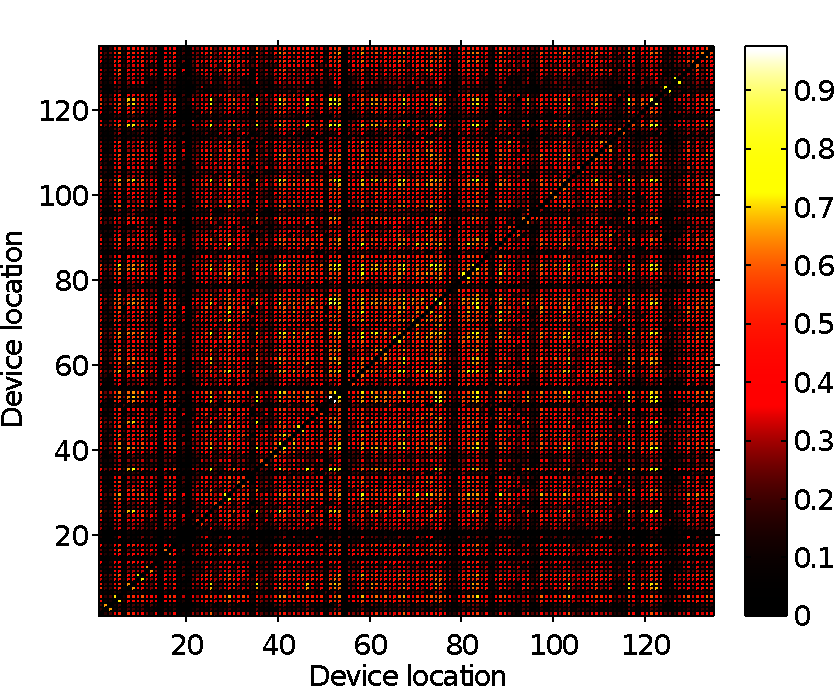
\includegraphics[width=.48\textwidth]{img/heatMap_raw_201106-eps-converted-to.pdf}}\\
\subfloat[High Frequencies\label{fig:heatmap:high}]{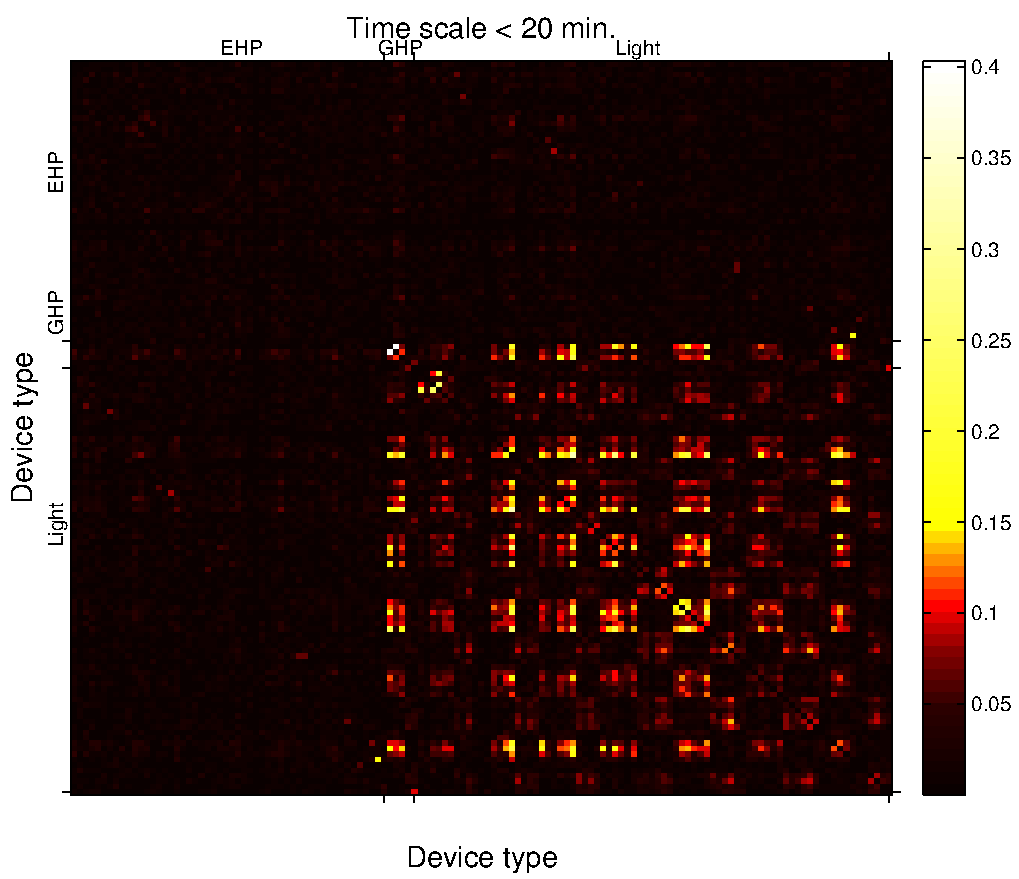
\includegraphics[width=.48\textwidth]{img/heatMap_1_201106-eps-converted-to.pdf}}\hfill
\subfloat[Medium Frequencies\label{fig:heatmap:med}]{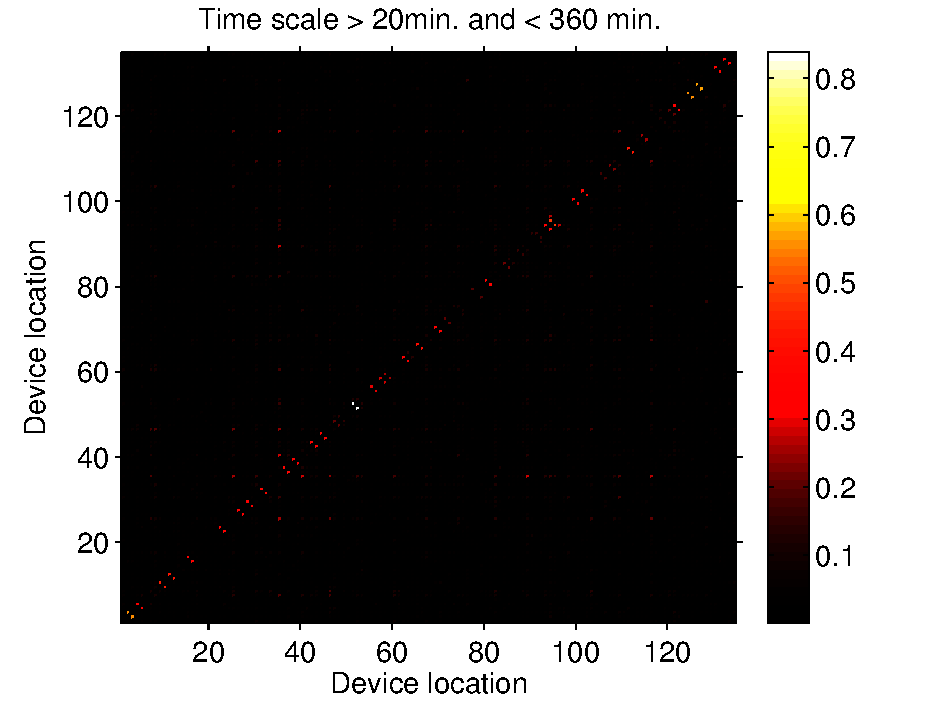
\includegraphics[width=.48\textwidth]{img/heatMap_2_201106-eps-converted-to.pdf}}\\
\subfloat[Low Frequencies\label{fig:heatmap:low}]{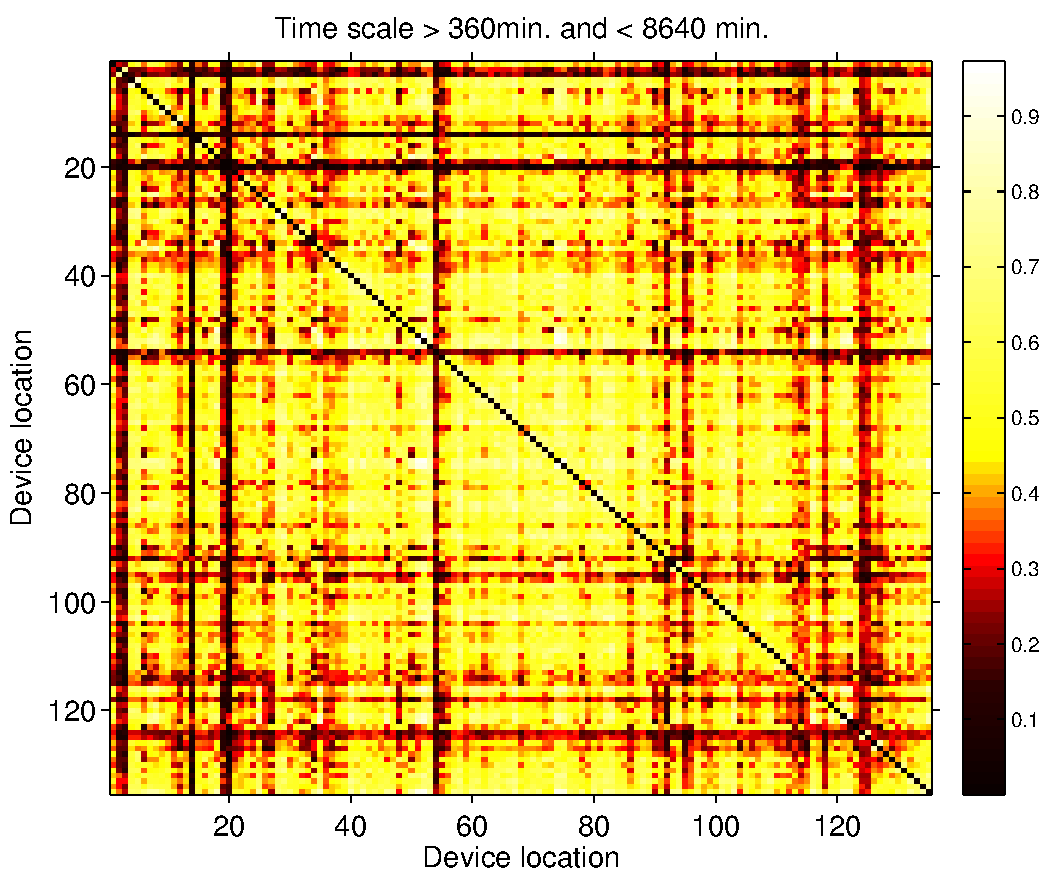
\includegraphics[width=.48\textwidth]{img/heatMap_3_201106-eps-converted-to.pdf}}\hfill
\subfloat[Residual data\label{fig:heatmap:res}]{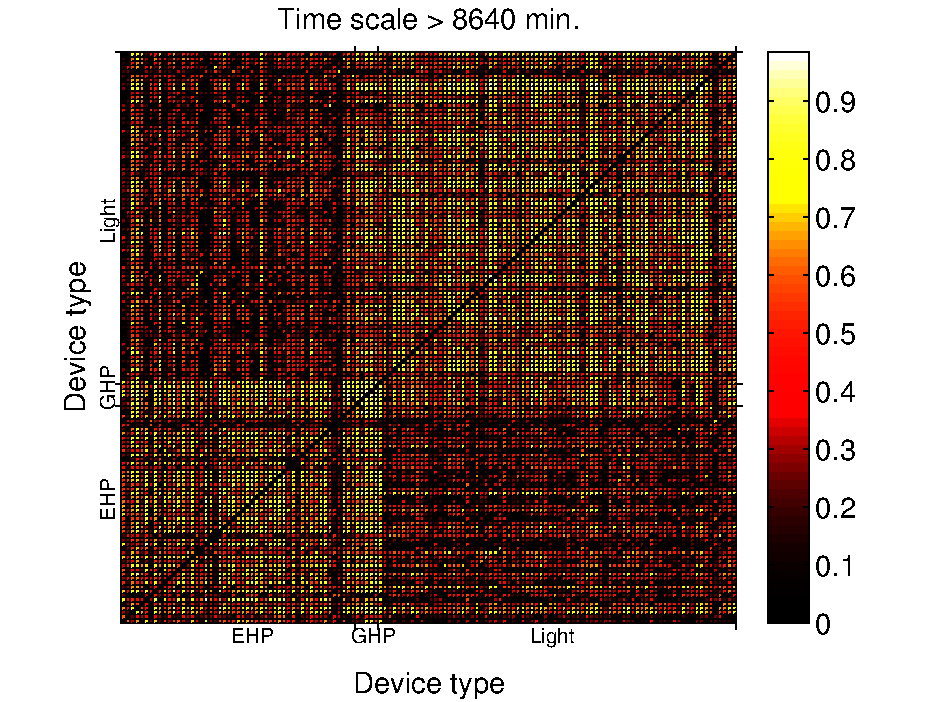
\includegraphics[width=.48\textwidth]{img/heatMap_4_201106-eps-converted-to.pdf}}
\caption{Reference correlation matrices for the four time scale ranges (the diagonal $x=y$ is colored in black for better reading). High correlation at the medium frequencies highlight devices that are located next to each other thus intrinsically related. Data at the low frequencies highlights the common daily pattern of the data. Unexpectedly the residual data permits to cluster devices of the similar type.}
\label{fig:heatmap}
\end{figure*}

\subsection{Devices behavior at different time scales}
The intrinsic-correlation estimator is evaluated using the data from the Engineering Building 2 as ground truth data.
As discussed in Section \ref{data:engbldg2} this dataset is appropriate to validate the proposed estimator as we assume that the lighting and air heating/cooling systems of the same room are intrinsically related.
Thereby we process the dataset using the proposed intrinsic-correlation estimator and verify that the correlation score assigned to the devices located in the same rooms are significantly high.

The dataset is split in 10 bins of 1 week long, for each bin all signals are processed with EMD and their correlation at the four distinct time scale is computed. 
Thereby, we obtain the four reference correlation matrices (i.e. the matrix of the median correlations) depicted in Figure \ref{fig:heatmap}.

\paragraph{High frequencies}
In this work the high frequencies correspond to the signals noise, therefore, we don't expect any beneficial information from the corresponding matrix.
Indeed in this experiments the corresponding reference matrix does not provide any help to discriminate devices location.
Thus, we emphasize that this data should be ignored in order to efficiently uncover the devices intrinsic relationship (contrarily to the approach proposed in \cite{romain:iotapp12}).
Interestingly, we found that the sensors monitoring the lighting systems generate consistent noise and could help one to cluster this type of sensor (Fig. \ref{fig:heatmap:high}).
  
\paragraph{Medium frequencies}
This article main interest is the data analysis at the medium frequencies as it is designed to capture the intrinsic device relationships.
Figure \ref{fig:heatmap:med} depicts the devices correlation at the medium frequencies, this is significantly different from the correlation matrix of raw signals (Fig. \ref{fig:heatmap:raw}) as higher correlation are mainly along the matrix diagonal. 
Since the devices serving the same or adjacent rooms are placed nearby in the matrix it confirms our assumption; high correlation scores at the medium frequency band stand for devices intrinsic relationship.
Thus, this matrix helps us to cluster devices that are used in concert.
For example using a community mining algorithm (i.e. the Louvain algorithm \cite{blondel:unfolding}) we identify the communities described by this reference matrix.
As expected we obtained mainly clusters of only two devices (light and HVAC serving the same room), but we also found clusters that are composed of more devices.
The biggest cluster contains 33 devices that are 2 GHP devices and the corresponding lights.
Similarly another cluster of 8 devices contains 1 GHP and the corresponding lights and the 2 other GHP are clustered together with a single light.
We also obtained a cluster containing the 3 HVAC serving the three server rooms. Although these server rooms are located at different floors the estimator measured a strong correlation between these devices as they are managed in the same way.
Interestingly we also observe a couple of clusters that consist of independent devices serving two adjacent rooms belonging to the same lab.
These clusters are the definite evidence of the proposed estimator ability to uncover devices intrinsic-relationships.
 
\paragraph{Low frequencies}
Low frequencies intend to capture the daily pattern common to all the devices.
Figure \ref{fig:heatmap:low} depicts the partial signals correlation coefficient at low frequencies, it is similar to the raw signals correlation matrix (Fig. \ref{fig:heatmap:raw})as it advertises no particular structure.
As expected the data in this time scale range feature similar characteristics thus most of the devices are highly correlated.
Therefore, for our purpose ignoring this data is relevant as it prevents to precise comparison of the devices utilization.
 
\paragraph{Residual data}
In this experiments the residual data stands for the weekly trend of the devices.
Obviously this data provides poor insights on the devices intrinsic-relationships.
But surprisingly by reordering the correlation matrix based on the device types (Figure \ref{fig:heatmap:res}) we found two major clusters of correlated devices.
The first cluster consists of HVAC devices (see EHP and GHP in Fig. \ref{fig:heatmap:res}) whereas the second one contains only light devices. 
An in-depth examination of the data revealed underlying trends that are inherent to the device types. 
For example, as the consumption of both the EHP and GHP devices is driven by the building occupancy and the outside temperature, these two types of devices follow the same long-range trend. 
However, the use of light is independent from the outside temperature thus the lighting systems follow a common trend that is different from the EHP and GHP one.
~\\

We conducted the same experiments by splitting the dataset in 70 bins of 1 day long and observed analogous results for short time scales but dissimilar for longer scales.
At high and medium frequencies we obtained very similar matrices, however, almost no data is captured at the low frequencies (because the bins are too short to exhibit daily oscillations) and the residual data captures only the daily trend that is irrelevant for discriminating the device types.

TODO add some info about the reference matrix for the Cory Hall?

\subsection{Anomalies}
We now evaluate the performance of the anomaly detector (Section \ref{methodo:ano}) with the data collected at the Engineering Building 2 and the one from the Cory Hall.
Nevertheless, due to the lack of ground truth data such as rooms schedule or reports of energy wastes evaluating the anomaly detector is not straightforward.

\paragraph{Evaluation process}
To validate the detector performance we manually inspect the identified anomalies.
Therefore, for each reported alarm $(t,i)$ we thoroughly investigate the data from the device $i$ and its related devices (as provided by the reference matrix) at the time bin $t$ in order to identify the root cause of the alarm.
In particular we retrieve the major relationship change that causes the anomaly (i.e. $\max(|w_j(C_{i,j}^t - R_{i,j})|)$, see Section \ref{methodo:ano}) and examine the metadata associated to the corresponding device $j$ and the sign of the relationship change $C_{i,j}^t - R_{i,j}$.
A positive relation change value means the devices correlation at the time bin $t$ is abnormally high, whereas negative value means that the relationship between the two devices is broken.

Furthermore, this investigation allow us to classify the alarms into five groups,
\begin{itemize}
 \item \emph{High power usage}: alarms standing for electricity wastes.
 \item \emph{Low power usage}: alarms caused by a device abnormal low electricity consumption.
 \item \emph{Punctual abnormal usage}: short term (less than 2.5 hours) raise or drop of the electricity consumption.
 \item \emph{Missing data}: alarms raised due to the hardware/software failures of sensors.
 \item \emph{Other}: Usually alarms whose root cause is unknown.
\end{itemize}

% However, the exhaustive enumeration of the true negatives (i.e. saving opportunities that are not detected) is impractical because of the size of the analyzed datasets (number of devices and traces length).
% Instead we exhibit the detector sensitivity by varying $\tau$, the threshold value.

\begin{figure}
\begin{center}
 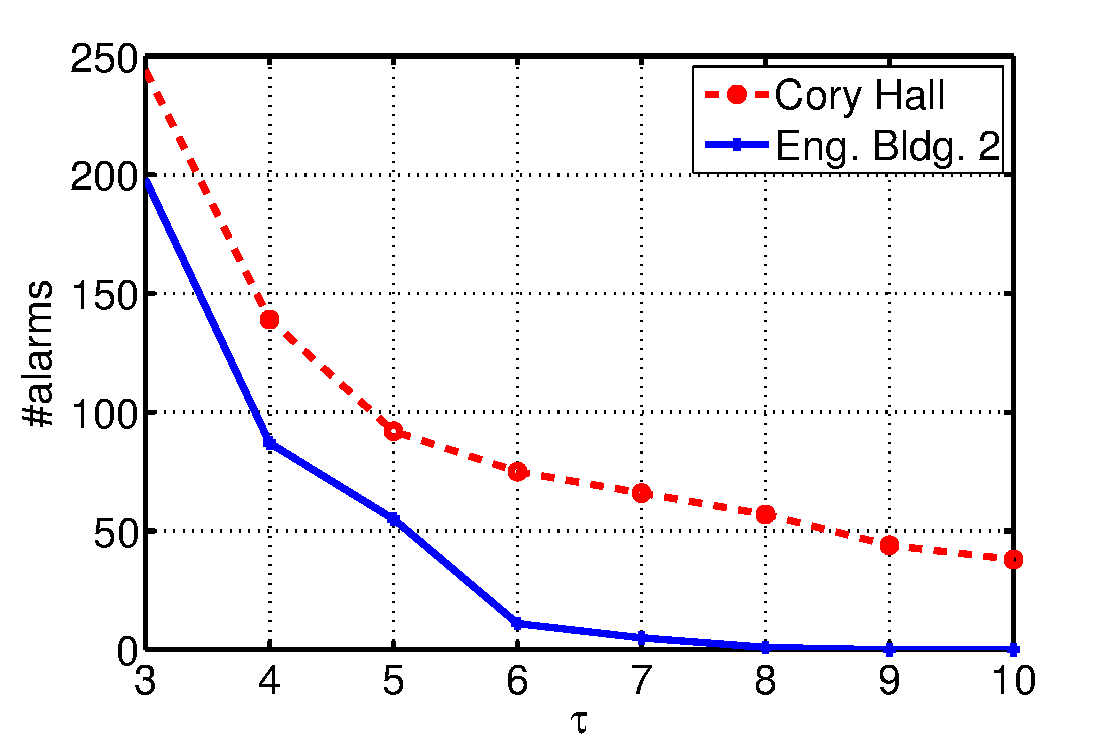
\includegraphics[width=.49\textwidth]{img/threshold-eps-converted-to.pdf}
 \caption{Number of reported alarms for various threshold value ($\tau=[3,10]$).}
 \label{fig:thres}
 \end{center}
\end{figure}

\paragraph{Experimental setup}
For all the experiments presented in this section the data is split in time bins of one day long.
% starting from 09:00 am which is approximately the offices opening hours.
% We particularly discourage to start the time bins at midnight as we found that numerous anomalies appear at night and they are better highlighted if they are not spanning two time bins.
The reference matrix is computed using all the time bins, then, its distance to each time bin is calculated.
As we seek for the abnormal changes of the devices intrinsic-relationships the anomaly detector process only the data at the medium frequencies and disregard all others time scales ranges.

\begin{figure*}[t]
  \subfloat[Broken relationship between devices from the same room $X_1$\label{fig:res:eng1}]{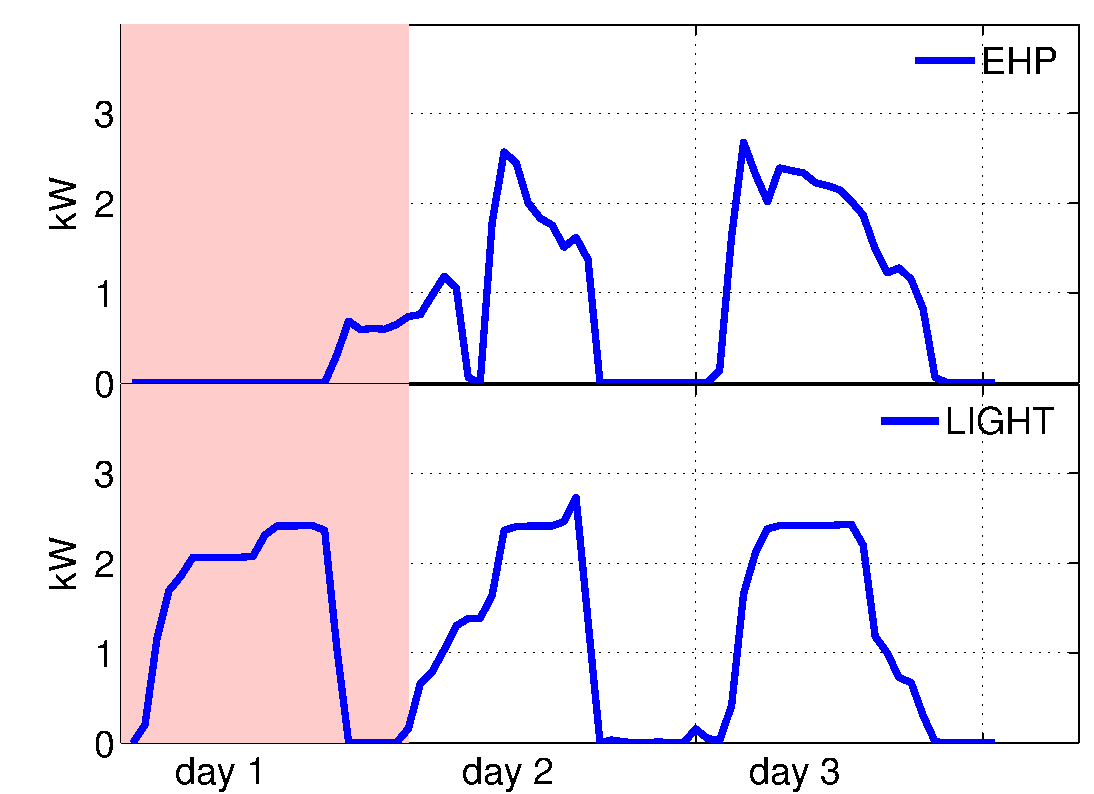
\includegraphics[width=.32\textwidth]{img/0sig20_sig31alarm1-eps-converted-to.pdf}} \hspace{.015\textwidth} %EHP turned on at night!?
  \subfloat[Broken relationship between devices from the same room $X_2$\label{fig:res:eng2}]{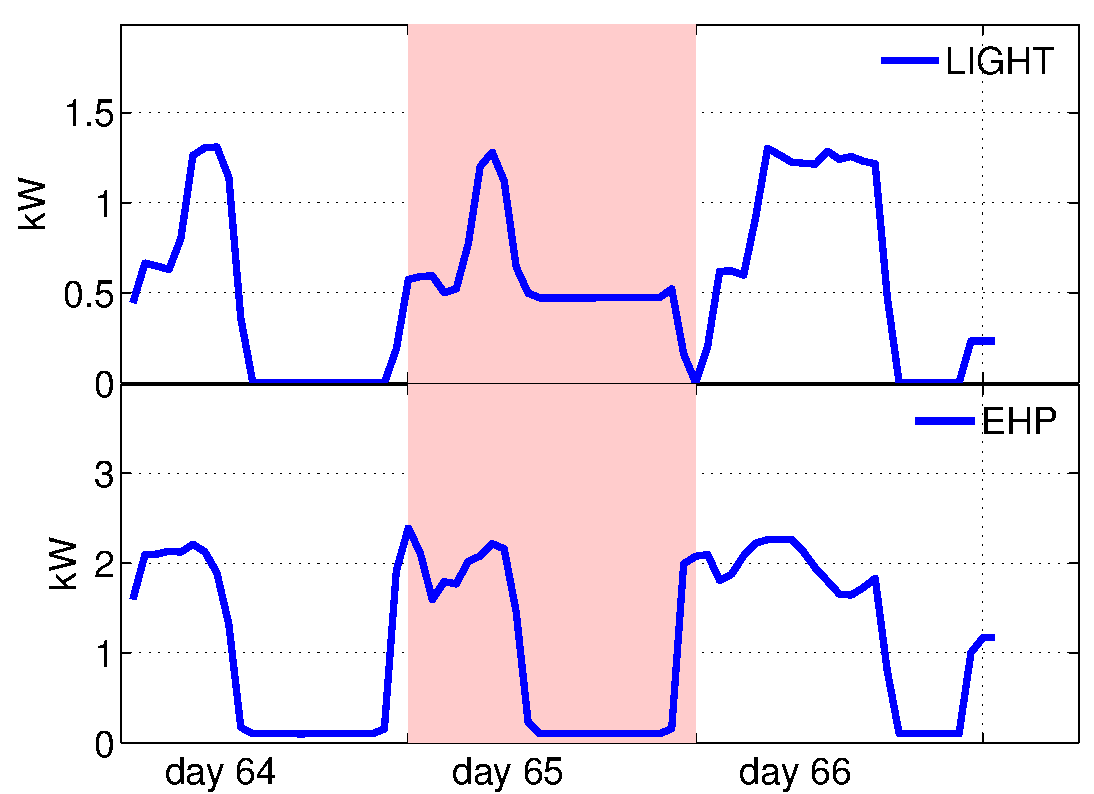
\includegraphics[width=.32\textwidth]{img/0sig134_sig123alarm65-eps-converted-to.pdf}} \hspace{.015\textwidth}  %Light left on during night
 \subfloat[Unexpected high correlation between devices from different rooms\label{fig:res:eng3}]{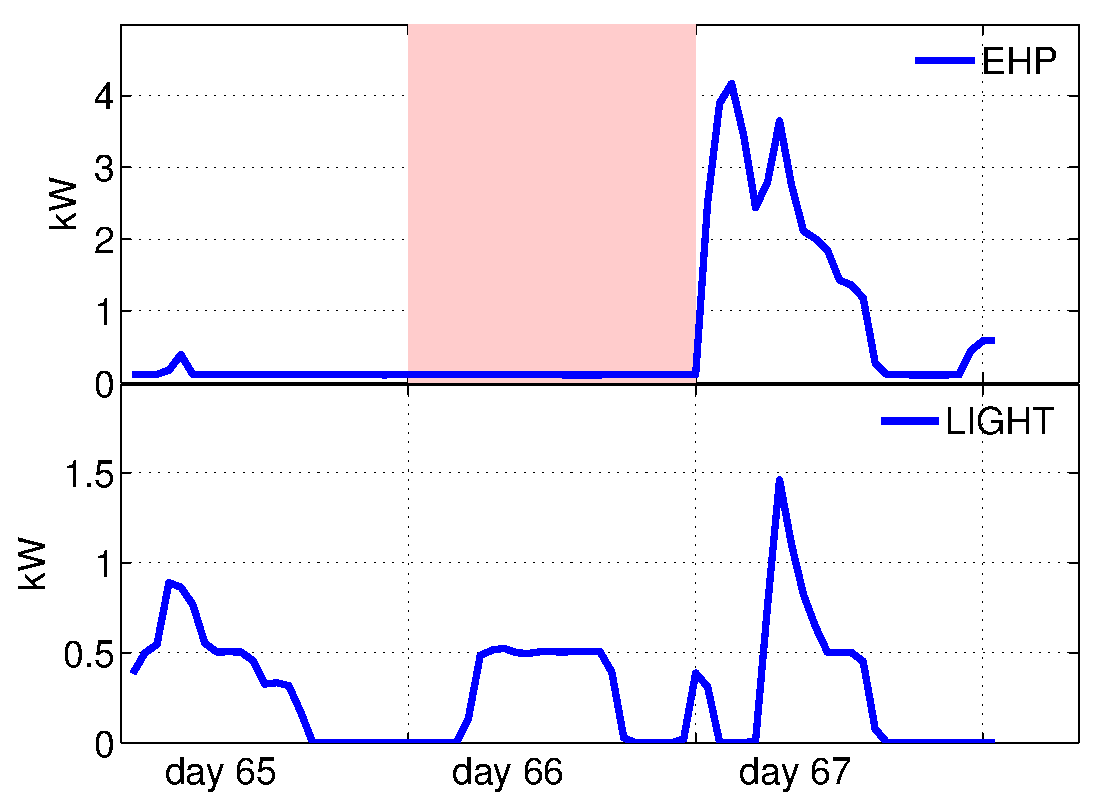
\includegraphics[width=.32\textwidth]{img/0sig24_sig33alarm66-eps-converted-to.pdf}}\\ %Three EHPs that are really correlated
 \subfloat[Long term anomaly partially detected\label{fig:res:eng4}]{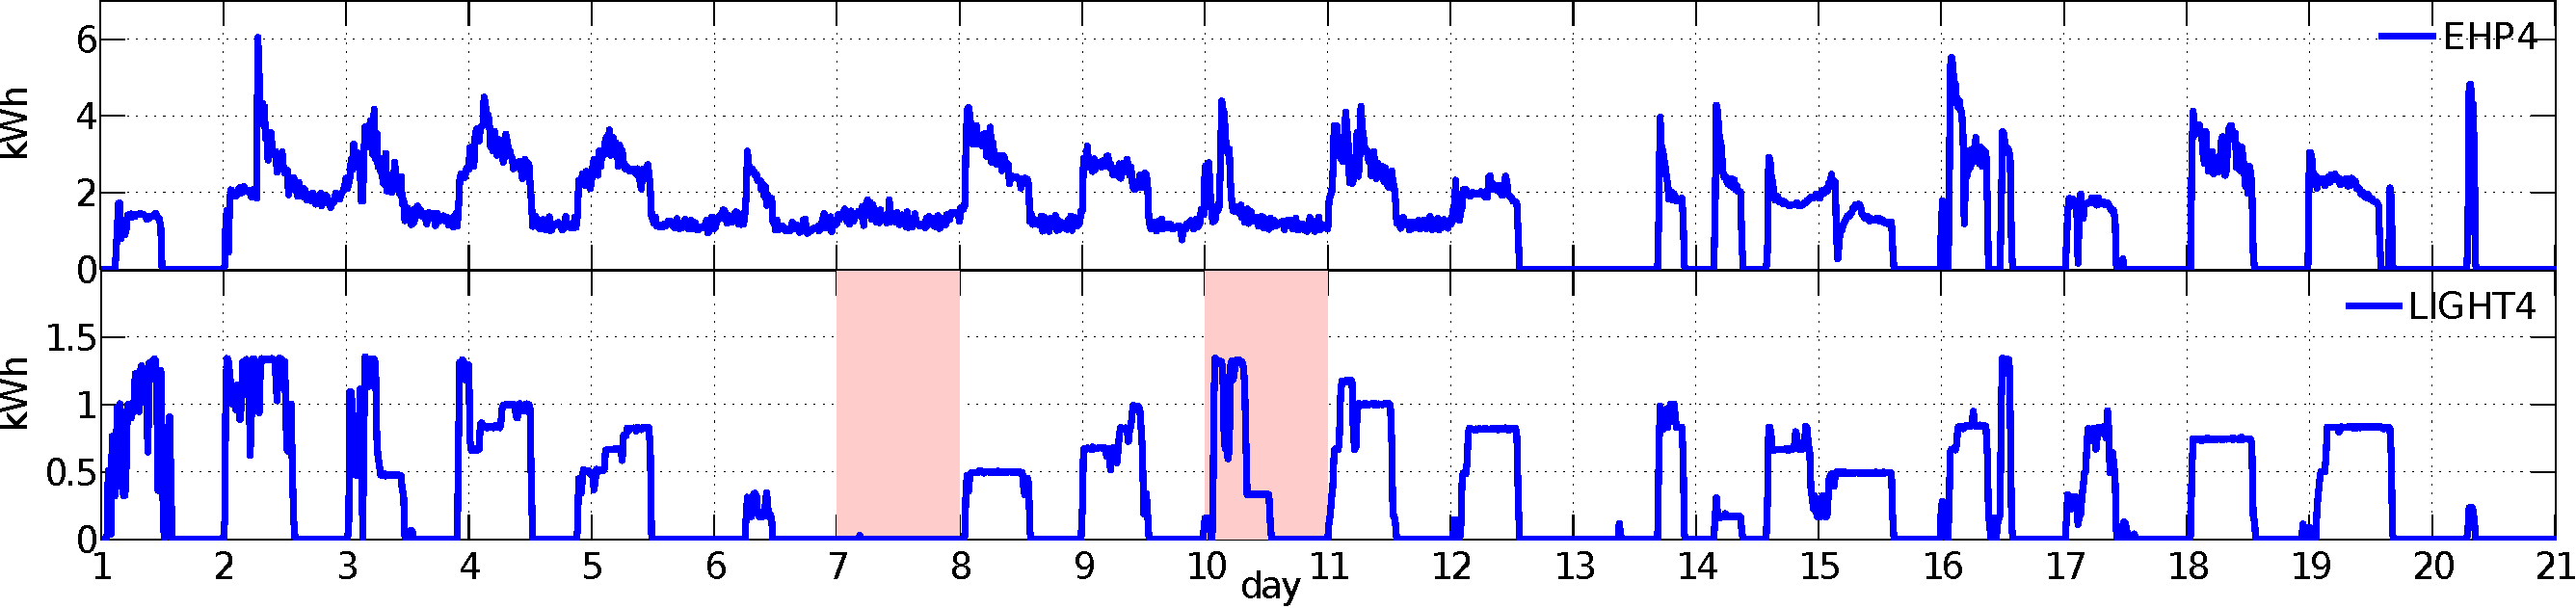
\includegraphics[width=\textwidth]{img/0sig3_sig15alarm7-eps-converted-to.pdf}}\\  
\caption{Example of alerts (red rectangles) reported by the anomaly detector using the Engineering Building 2 dataset}
\end{figure*}

By varying the threshold $\tau$ we can tune the sensitivity of the detector thus the number of reported alarms.  
Furthermore, by plotting the number of alarms against the value of $\tau$ for both datasets (Fig. \ref{fig:thres}) we observe an elbow in the graph around $\tau=5$.
With thresholds lower than this pivot value ($tau<5$) the number of alarms is significantly increasing thus likely to report less important anomalies, whereas, for higher value ($\tau>5$) the number of alarms is slowly decreasing thus provide a more conservative result that only consists of the most important anomalies.
As this pivot value is usually a good trade off we set $\tau=5$ for both datasets.


\subsubsection{Engineering Building 2}

\begin{table}
\begin{center}
\begin{tabular}{|l||c|c|c|c|c|}
\hline
Dataset&High&Low&Punc.&Missing&Other\\ \hline \hline
Eng. Bld. 2& 9 & 6 & 1 & 36 & 3 \\ \hline
Cory Hall& 25 & 7 & 4 & 0 & 3 \\ \hline
\end{tabular}
\end{center}
\caption{Alarms classification result for both dataset.}
\label{tab:classif}
\end{table}

The anomaly detector reported 55 alarms along the 10 weeks of the Engineering Building 2 dataset.
However, 36 alarms are discarded as they stand for missing data in the dataset; one GHP has no data for the first 18 days.
Since this device is highly correlated to another GHP in the reference matrix, their relationship is broken for the 18 first bins and two alarms per bin are raised (one for each GHP).

In spite of the university measures to reduce its electricity footprint, the detector reported 9 alarms usually standing for small electricity wastes (Table \ref{tab:classif}).
For example Figure \ref{fig:res:eng1} depicts the electricity consumption of the light and HVAC system of the same room for which two alarms have been raised at the first time bin.
Because the HVAC was not used during daytime but has been turned on at night when the light is turned off the relationship between the two devices is broken and an alarm is raised for each device.
Figure \ref{fig:res:eng2} is another example of energy waste where the light has been left on during night whereas the HVAC has been turned off.
The top-priority anomaly reported by the detector is caused by the 10 days long constant use of a room HVAC (Figure \ref{fig:res:eng4}) and this opportunity to save electricity account for 165 kWh.
The detector partially reported this anomaly, however, lower threshold value $\tau$ permits to identify most of it.

\begin{figure*}[t]
  \subfloat[Cooler failure\label{fig:res:cory1}]{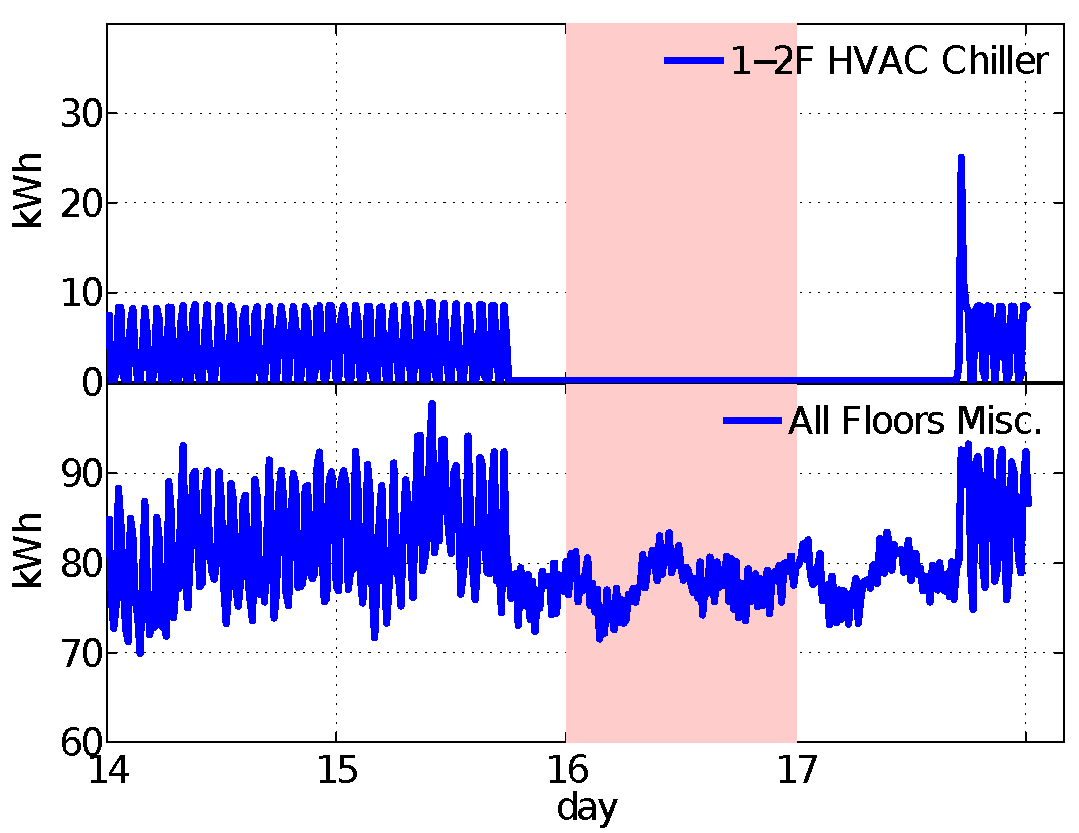
\includegraphics[width=.32\textwidth]{img/1sig37_sig55alarm16-eps-converted-to.pdf}} \hspace{.015\textwidth}
 \subfloat[Abnormal usage\label{fig:res:cory21}]{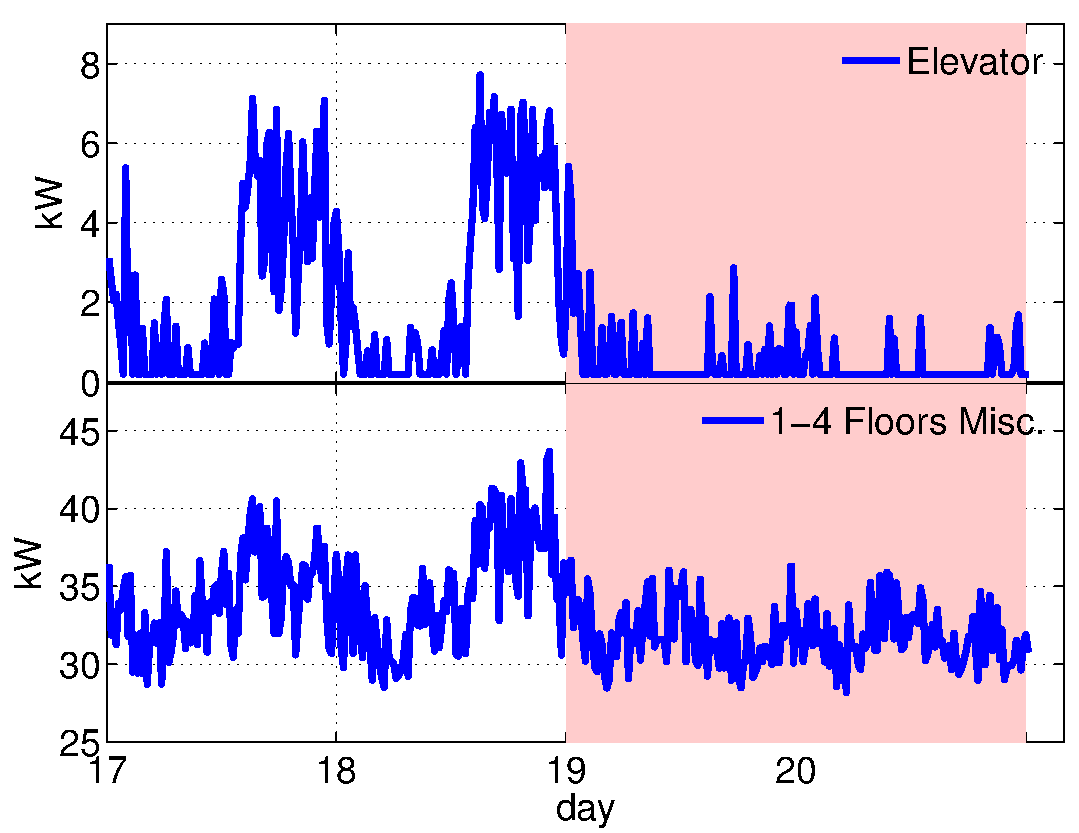
\includegraphics[width=.32\textwidth]{img/1sig7_sig49alarm19-eps-converted-to.pdf}}
 \hspace{.015\textwidth}
 \subfloat[Normal usage\label{fig:res:cory22}]{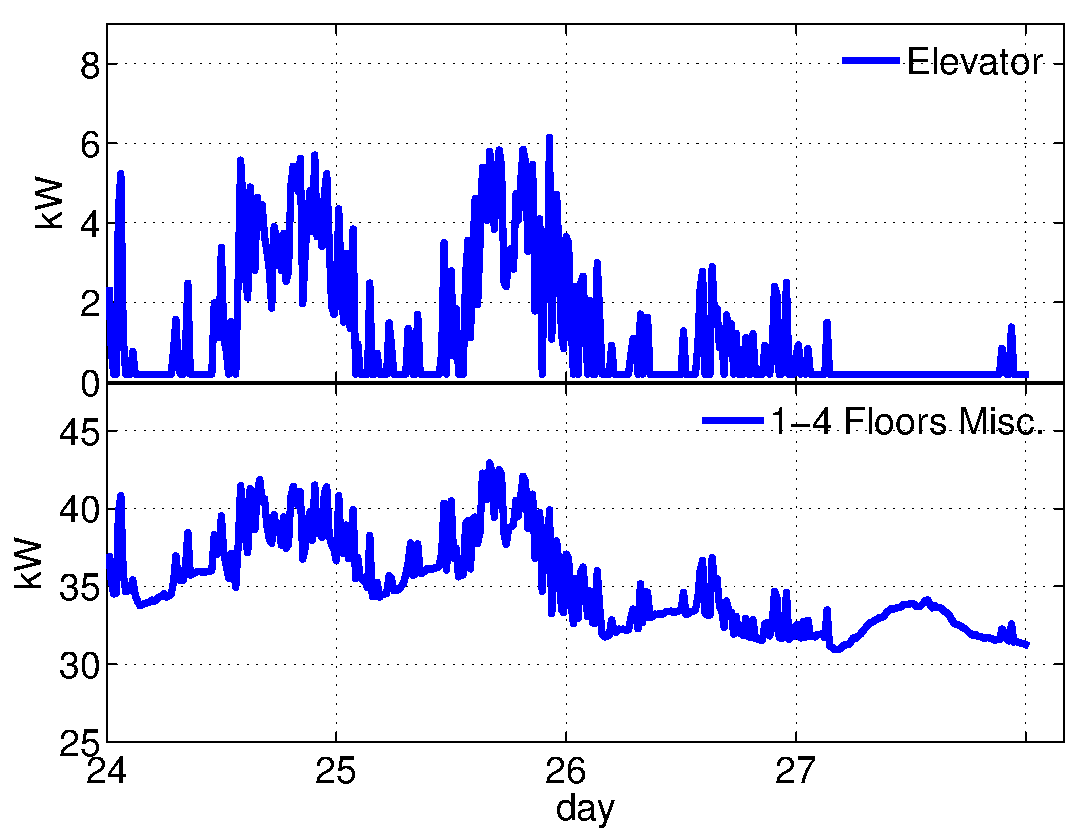
\includegraphics[width=.32\textwidth]{img/1sig7_sig49alarm-eps-converted-to.pdf}}\\ 
 \subfloat[Heating/cooling anomaly\label{fig:res:cory3}]{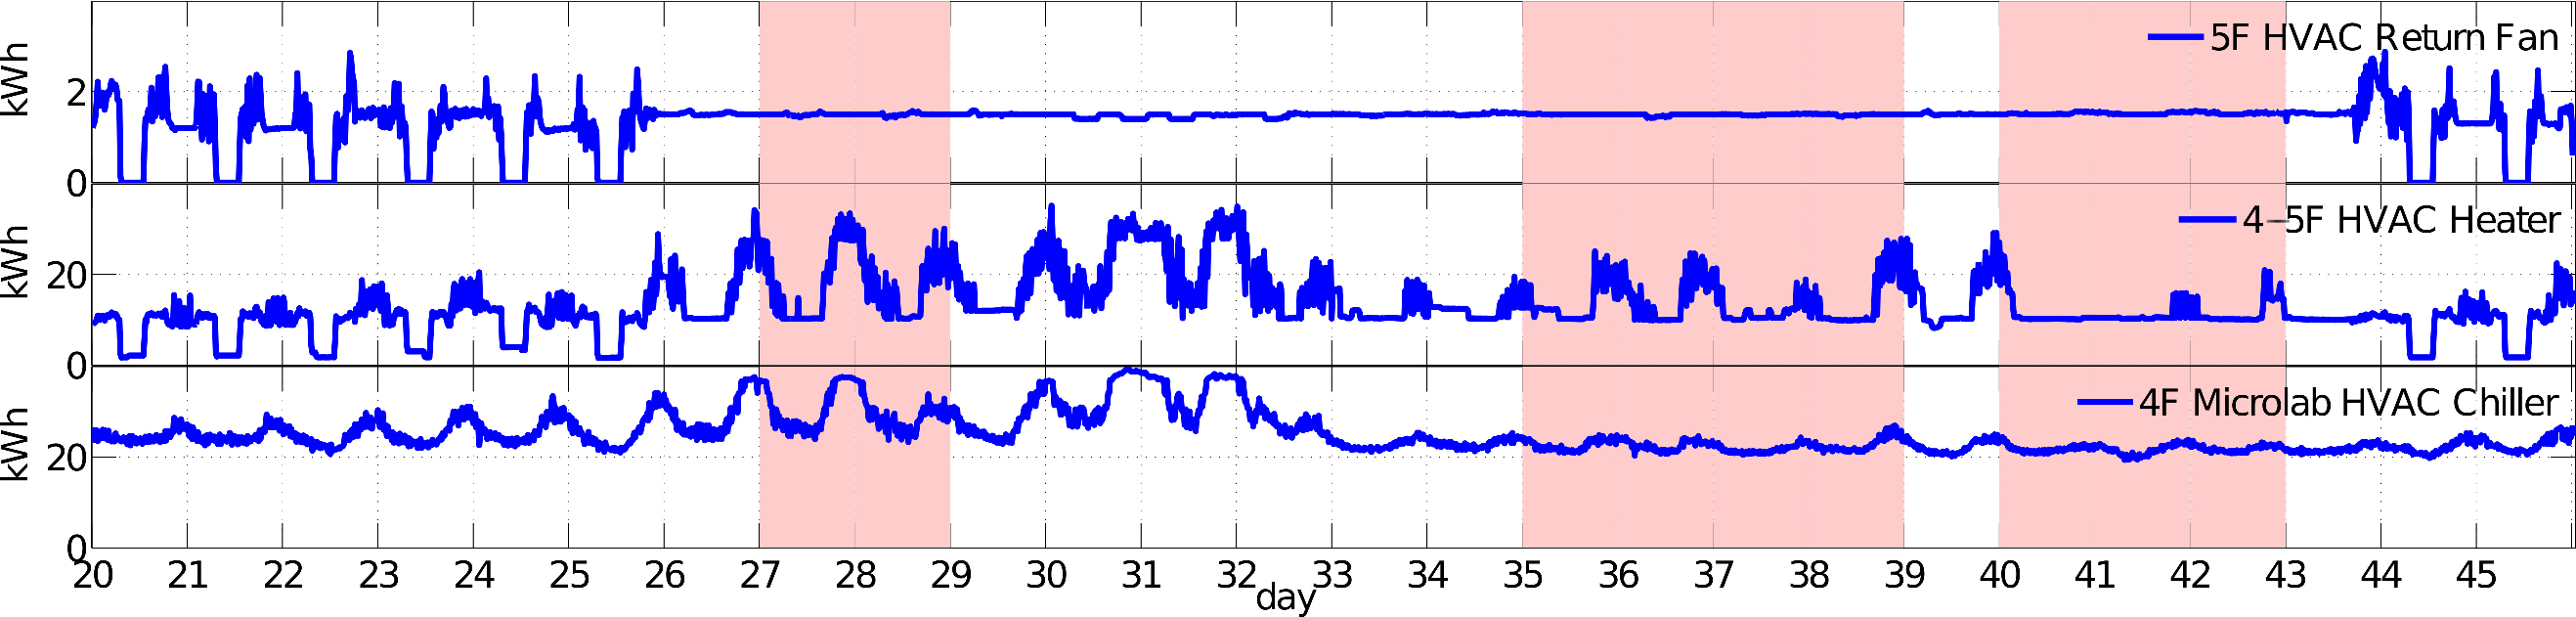
\includegraphics[width=\textwidth]{img/1sig34_sig54alarm27-eps-converted-to.pdf}} 
\caption{Example of anomalies identified by the proposed detector for the Cory Hall dataset}
\end{figure*}

6 alarms reported abnormal low power usage, our inspection revealed that they usually correspond to saving initiatives from the rooms users probably due to the electricity concern in Japan.
This behavior is depicted in Figure \ref{fig:res:eng3}, the occupancy is obvious as the light is used at the usual office hours but the air conditioner has not been tuned on during in the sole intention to save electricity.

\subsubsection{Cory Hall}
The proposed anomaly detector reported 39 alarms for the Cory Hall dataset (Table \ref{tab:classif}).
Among these alarms 7 are classified as low power usage, however, our inspection revealed that the root causes for this type of anomaly is different than for the Engineering Building 2 dataset.
For the previous experiment this type of anomaly stands mainly for saving measures from the room user, however, in this case we observe that the low power usage usually stands for device failures or misconfigurations.
For example, Figure \ref{fig:res:cory1} depicts the electricity consumption of the 2nd floor chiller and at a power riser that includes the consumption of multiple systems including the chiller.
As the chiller suddenly stops working the correlation between both measurements is significantly altered and an alarm for each device is raised.

The detector also reported 25 alarms corresponding to high power usage. 
Interestingly, we indirectly observed a saving opportunity from the measurements of the elevator power consumption and a power panel that provides electricity to facilities from the 1st to the 4th floor.
Figure \ref{fig:res:cory21} and \ref{fig:res:cory22} shows the electricity consumption for these two devices. 
We found that the elevator is a good occupancy indicator as the amount of electricity going through the panel fluctuates along with the elevator power consumption (Figure \ref{fig:res:cory22}).
However, the detector identified anomalous activity during a week-end, in this case the electricity consumption measured at the panel is independent from the elevator usage and oscillates significantly.
Since the particular device causing this anomaly is not instrumented with a sensor we could not precisely identified the root cause of this anomaly.

The most important anomaly identified by the detector is shown in Figure \ref{fig:res:cory3}.
This anomaly corresponds to the malfunctioning of the HVAC Heater serving the 4th and 5th floor. 
In fact the heater is constantly working for 18 consecutive days thus over provisioning the corresponding floors.
This also results in the increase of the 4th floor HVAC Chiller power consumption to maintain appropriate temperature.
This situation where heating and cooling system are competing is a well-know problem in building management as it leads to important energy wastes.
For this particular example the heater only electricity waste is estimated around 2300 kWh which is 3.7 times the mean electric consumption of the Cory Hall.
Nevertheless, as the anomaly spans over 18 days it is hidden in the building overall consumption thus difficult to be detected by building administrators without the help of the proposed method.
